\documentclass{classrep}
\usepackage[utf8]{inputenc}
\usepackage{color}
\usepackage{makecell}
\usepackage{graphicx}
\usepackage{url}
\usepackage{hyperref}

\studycycle{Informatyka, studia STACJONARNE, I st.}
\coursesemester{VI}

\coursename{Komputerowe systemy rozpoznawania}
\courseyear{2020/2021}

\courseteacher{prof. dr hab. inż. Adam Niewiadomski}
\coursegroup{poniedziałek, 12:00}

\author{
  \studentinfo{Julia Szymańska}{224441} \and
  \studentinfo{Przemysław Zdrzalik}{224466} }

\title{Projekt 1. Klasyfikacja dokumentów tekstowych}
\usepackage{multirow}
\begin{document}
\maketitle


\section{Cel projektu}
Celem projektu jest stworzenie aplikacji klasyfikującej zadany zbiór danych tekstowych metodą K najbliższych sąsiadów (k-NN). Aplikacja ma za zadanie dokonać ekstrakcji cech na zbiorach tekstów\cite{dane} oraz następnie dokonać ich klasyfikacji.\\


\section{Klasyfikacja nadzorowana metodą $k$-NN}


Metoda K najbliższych sąsiadów, w skrócie metoda $k$-NN\cite{dane}, jest to algorytm stosowany do klasyfikacji, który nie wymaga etapu uczenia. 
Polega na zaklasyfikowaniu rozpatrywanego elementu do grupy ze zbioru uczącego, gdzie spośród k najbliższych rozpatrywanemu elementowi sąsiadów najwięcej z nich należy do tej grupy. Klasyfikator przyjmuje cztery parametry wejściowe takie jak: warotść k - ilość rozpatrywanych sąsiadów, proporcje podziału zbiorów na zbior uczący i zbiór testowy, zbiór cech, a także metrykę i/lub miarę prawdopodobieństwa. Wynikiem klasyfikacji jest zaklasyfikowanie elementu do jednego ze zbiorów uczących. 


\subsection{Ekstrakcja cech, wektory cech}
Na zbiorach danych tekstowych należy dokonać ekstrakcji cech, które będą wartościami rzeczywistymi oraz tekstowymi. Dane cechy będą reprezentowały tekst w postaci wektora cech podczas procesu klasyfikacji. Przed dokonaniem ekstrakcji cech, z tekstów usuwane są słowa znajdujące się na stop liście. Teksty ze zbioru danych tekstowych posiadają strukturę: \begin{equation}
  \begin{array}{l}
  <TEXT> \\
\;\;\;\; <TITLE/>\\
\;\;\;\; <AUTHOR/>\\
\;\;\;\; <DATELINE/>\\
 \;\;\;\;<BODY/> \\
</TEXT>
  \end{array}
\end{equation}\\
\begin{enumerate}
  \item Liczba słów - cecha ta oznacza liczbę słów które składają się na pobrany tekst. Cecha ta będzie charakteryzowała długość dokumentu w postaci liczby całkowitej \begin{equation}  c_1 = len \end{equation} gdzie len - liczba słów w tekście.\\
 
 
 \item Data z tagu  \textless Dateline\textgreater\ - Każdy tekst w swoim body posiada tag \textless Dateline\textgreater , w którym znajduje się miasto oraz data podana w postaci miesiąca i dnia. Data będzie konwertowana na wartość liczbową, gdzie liczbą tą będzie numer podanego dnia w ciągu roku, licząc rok tak jakby rok był rokiem przestępnym, przykładowo data 1 marca będzie reprezentowana poprzez wartość 61. Cechę traktujemy jako cechę w postaci liczby całkowitej. Wartość będzie oznaczana poprzez symbol  c\textsubscript{3}.    \\
  \item Lokacja z tagu \textless Dateline\textgreater - jak wyżej. Lokację traktujemy jako cechę tekstową. Wartość będzie oznaczana poprzez symbol  c\textsubscript{4}. \\
  \item Tytuł z tagu \textless Title\textgreater - Każdy tekst w swoim body posiada tag \textless Title\textgreater. Tytuł traktujemy jako cechę tekstową. Wartość będzie oznaczana poprzez symbol  c\textsubscript{5}.\\
  \item Autor z tagu \textless Author\textgreater - Większość tekstów w swoim body posiada tag \textless Author\textgreater. Autora traktujemy jako cechę tekstową. Wartość będzie oznaczana poprzez symbol  c\textsubscript{6}.\\
  \item Najczęściej występująca nazwa kraju - wybieramy najczęściej występującą w analizowanym tekście nazwę kraju. Nazwy krajów pobieramy z dołączonego pliku all-places-strings.lc, przykładowo krajem występującym w pliku jest 'albania'.Nazwę kraju traktujemy jako cechę tekstową.Wartość będzie oznaczana poprzez symbol  c\textsubscript{7}.\\
  \item Zbiór występujących słów kluczowych. Za słowa kluczowe przyjmujemy słowa znajdujące się w dołączonych plikach o rozszerzeniach .lc.txt. Cechę traktujemy jako cechę tekstową.  \begin{equation}  c_8 : c_8 \in N \cap t \end{equation} gdzie N - zbiór wszystkich słów kluczowych, t - zbiór słów należących do tekstu\\
  \item Liczba wystąpień słów kluczowych - traktujemy jako cechę w postaci liczby całkowitej.\begin{equation}  c_9 = | c_8 | \end{equation} gdzie c\textsubscript{8} - zbiór występujących słów kluczowych\\
  \item Nasycenie tekstu ilością słów kluczowych - traktujemy jako cechę w postaci liczby zmienno przecinkowej.  \begin{equation} c_{10} = c_9 / c_1 \end{equation}  gdzie c\textsubscript{9} - ilość wystąpień słów kluczowych w tekscie, c\textsubscript{1} - liczba słów w tekście\\
  \item Najczęściej występujące słowo kluczowe - wybieramy najczęściej występujące w analizowanym tekście słowo kluczowe. Cechę traktujemy jako cechę tekstową. Wartość będzie oznaczana poprzez symbol  c\textsubscript{11}.\\
  \item Liczba unikatowych słów - zliczamy liczbę unikatowych słów, to znaczy występujących dokładnie raz w analizowanym tekście. Cechę traktujemy jako cechę w postaci liczby całkowitej. Wartość będzie oznaczana poprzez symbol  c\textsubscript{12}.\\
\end{enumerate}

\ \\ \\
Wektor cech będzie reprezentowany w postaci: 

\begin{equation} w = [c_1, c_2, c_3, c_4, c_5, c_6, c_7, c_8, c_9, c_{10}, c_{11}, c_{12}] \end{equation}



\subsection{Miary jakości klasyfikacji} 
W celu określenia jakości wykonanej klasyfikacji korzystamy z czterech miar jakości klasyfikacji. Aby obliczyć każdą z miar tworzymy tablicę pomyłek, inaczej macierz błędu \cite{tablica}. Tablica składa się z dwóch wierszy i dwóch kolumn, gdzie wiersze to klasy predykowane, a kolumny to klasy rzeczywiste. Dane oznaczone jako dane pozytywne i negatywne poddawane są klasyfikacji, która przypisuje im predykowaną klasę pozytywną bądź negatywną.\\

\begin{table}[h!]
\begin{tabular}{l|l|c|c|c}
\multicolumn{2}{c}{}&\multicolumn{2}{c}{Klasa rzeczywista}&\\
\cline{3-4}
\multicolumn{2}{c|}{}&Pozytywna&Negatywna&\multicolumn{1}{c}{}\\
\cline{2-4}
\multirow{2}{*}{\thead{Klasa\\ predykowana} }& Pozytywna&  \thead{prawdziwie\\ pozytywna (TP)}
 & \thead{fałszywie\\ pozytywna (FP)} \\
\cline{2-4}
& Negatywna & \thead{prawdziwie\\ negatywna (TN)} & \thead{fałszywie\\ negatywna (FN)} \\
\cline{2-4}
\end{tabular}
 \caption{Wzór tablicy pomyłek.}
\end{table}


Stosowane miary jakości klasyfikacji:\\
\begin{itemize}
  \item Dokładność (ang. accurancy), ACC  - jest to stopień zgodności wartości ze średnią arytmetyczną uzyskanych wyników. \begin{equation} ACC = (TP + TN)/(TP + FN + FP + TN)  \end{equation}
 \item Precyzja (ang. precision), PPV  - jest to stopień zgodności wyników uzyskanych w określonych warunkach z wielokrotnych pomiarów. \begin{equation} PPV =  TP / (TP+FP) \end{equation}
\item Czułość (ang. recall), TPR  - jest to stosunek wyników prawdziwie dodatnich do sumy prawdziwie dodatnich i fałszywie ujemnych. \begin{equation}   TPR = TP / (TP + FN) \end{equation}
\item Swoistość (ang. specificity), TNR   - jest to stopień zgodności wartości ze średnią arytmetyczną uzyskanych wyników. \begin{equation} TNR = TN / (FP + TN) \end{equation}
\end{itemize}


\section{Klasyfikacja z użyciem metryk i miar podobieństwa tekstów}
W procesie klasyfikacji możliwe jest wykorzystanie jedne z trzch metryk: Metryka Euklidesowa, Metryka Czebyszewa, Metryka Uliczna. Metryki służą obliczeniu odległości pomiędzy dwoma wektora o dowolnym rozmiarze.\\\\ Metryka Eukliedesowa\cite{dane} jest opisana wzorem: 
\begin{equation} d(x, y) = \sqrt{(y_1 - x_1)^2 + ... + (y_n - x_n)^2}  \end{equation}
gdzie: d(x, y) - odległość pomiędzy wektorem x i y; x, y - wektory o tym samym rozmiarze; n - rozmiar wektorów x i y;  x\textsubscript{n}, y\textsubscript{n} - składowe wektora. 
\\\\
Metryka Czebyszewa\cite{dane} jest opisana wzorem: 
\begin{equation} d(x, y) = max(|y_i - x_i|) \end{equation}
gdzie: d(x, y) - odległość pomiędzy wektorem x i y; x, y - wektory o tym samym rozmiarze; n - rozmiar wektorów x i y;  x\textsubscript{i}, y\textsubscript{i} - i-ta składowa wektora;
\\\\
Metryka Uliczna\cite{dane} jest opisana wzorem: 
\begin{equation} d(x, y) = \sum_{i = 1}^{n} |x_i - y_i| \end{equation}
gdzie: d(x, y) - odległość pomiędzy wektorem x i y; x, y - wektory o tym samym rozmiarze; n - rozmiar wektorów x i y;  x\textsubscript{n}, y\textsubscript{n} - składowe wektora. 
\\\\
By móc obliczyć odległość pomiędzy wektorami cech zadanych tekstów, należy wcześniej skorzystać z miar podobieństwa tekstu by zamienić tekst na liczbę w wektorach. W programie zostało użyte podobieństwo cosinusowe\cite{wyklad}. Należy utworzyć po jedym wektorze dla każdego z dwóch rozpatrywanych tekstów - x = \{ x\textsubscript{1}, x\textsubscript{2}, ... , x\textsubscript{n} \},  y = \{ y\textsubscript{1}, y\textsubscript{2}, ... , y\textsubscript{n} \}, gdzie x\textsubscript{n}, y\textsubscript{n}  to ilość wystąpień n-tego słowa, ze zbioru wszystkich słów występujących w tekstach cech obu wektorów, w zadanej cesze wektora cech. Dla tak utworzonych wektrów liczony jest kosinus kąta pomiędzy nimi ze wzoru:
\begin{equation} r_{cos} = \frac{\sum_{i = 1}^{n} x y}{\sqrt{\sum_{i = 1}^{n} x^2}\sqrt{\sum_{i = 1}^{n} y^2}} \end{equation}
gdzie r\textsubscript{cos} - to cos kąta pomiędzy wektorem x i y; x, y - rozpatrywane wektory; n - długość wektora.
\newline
Porównanie wyników klasyfikacji metody k-NN dla 10 różnych wartości parametru k. Pozostałe parametry pozostają niezmienne - proporcje podziału zbioru wektrów na zbiór treningowy i zbiór testowy - 80/20, a wybrana metryka to metryka Euklidesowa. 

\begin{table}[h!]
 \caption{Wstępne wyniki klasyfikacji dla różnych proporcji podziału zbioru wektrów na zbiór treningowy i zbiór testowy.}
 \centering
 \vspace{0.1cm}
 \begin{tabular}{c c}
  \textbf{Wartość k} & \textbf{Dokładność klasyfikacji -Accurancy}\\
\hline
  1 &  0.5926966292134831\\
  2 &   0.6713483146067416\\
  3 &  0.6629213483146067\\
  4 &  0.6657303370786517\\
  5 &  0.6741573033707865\\
  7 & 0.6657303370786517\\
  8 &  0.6741573033707865\\
  9 &   0.6741573033707865\\
 13  & 0.6629213483146067\\
200 &   0.6769662921348315 \\
 \end{tabular}
 \label{wyniki klasyfikacji dla różnych proporcji podziału zbioru wektrów na zbiór treningowy i zbiór testowy.}
\end{table}

Różne wartości parametru k nie mają znacznego znaczenia dal dokładności klasyfikacji. Najgorszy wynik był dla wartości parametru 1. Pozostałe wartości miały bardzo podobną dokładność klasyfikacji. 

\newpage
Kolejne porównanie jest dla różnych stosunków zbiorów uczących i testowych. Pozostałe parametry pozostają niezmienne - wartość parametru k to 2, a wybrana metryka to metryka Euklidesowa.


\begin{table}[h!]
 \caption{Wstępne wyniki klasyfikacji dla różnych 10 warotści parametru k.}
 \centering
 \vspace{0.1cm}
 \begin{tabular}{c c}
  \textbf{Stosunek zbioru treningowego do testowego} & \textbf{Dokładność klasyfikacji -Accurancy}\\
\hline
  1/99 & 0.45224719101123595\\
  20/80 &  0.648876404494382\\
  50/50 &  0.6713483146067416\\
  70/30 &  0.6629213483146067\\
  80/20 &  0.6348314606741573\\
 \end{tabular}
 \label{wyniki klasyfikacji dla roznych 10 wartosci parametru k}
\end{table}

Najgorzej wypadającym stosunkiem zbiorów uczących i testowych, gdzie stosunek wynosił 1/99, taki wynik został uzyskanu ponieważ mała ilość danych trenujących wpływa niekorzystnie na wyniki klasyfikacji. Najlepszy wynik był dla stosunku 50/50. 

Następne porównanie jest dla różnych metryk. Pozostałe parametry pozostają niezmienne - wartość parametru k to 1, proporcje podziału zbioru wektrów na zbiór treningowy i zbiór testowy - 50/50. 

\begin{table}[h!]
 \caption{Wstępne wyniki klasyfikacji dla różnych 3 różnych metryk.}
 \centering
 \vspace{0.1cm}
 \begin{tabular}{c c}
  \textbf{Metryka} & \textbf{Dokładność klasyfikacji -Accurancy}\\
\hline
  Euklidesowa &0.5758426966292135\\
  Czebyszewa & 0.5702247191011236\\
  Uliczna & 0.6235955056179775\\
 \end{tabular}
 \label{wyniki klasyfikacji dla roznych 10 wartosci parametru k}
\end{table}

Metryka Euklidesowa i Metryka Czebyszwa uzyskały podobny wynik jakości klasyfikacji. Metryka uliczna uzyskała najlepszy wynik. 

Kolejne porównanie polega na porównaniu wpływu różnych cech na wyniki jakości klasyfikacji. W tym celu wybieramy 4 zestawy różnych cech. 
\begin{enumerate}
\item Lokalizacja z tagu Dateline, data z tagu Dateline, tytul z tagu Title, autor z tagu Author
\item Najczęściej występujące słowo kluczowe, nasycenie tekstu słowami kluczowymi, liczba słów kluczowych, zbiór słów kluczowych
\item Długość tekstu, najczęściej występująca nazwa kraju, liczba unikatowych słów, 
\item Długość tekstu, lokalizacja z tagu dateline, zbiór słów kluczowych, najczęściej występująca nazwa kraju
\item Tytuł z tagu Title
\item Lokalizacja z tagu Dateline
\item Tytuł z tagu Title, lokalizacja z tagu Dateline
\end{enumerate}

Pozostałe parametry pozostają niezmienne - wartość parametru k to 2, proporcje podziału zbioru wektrów na zbiór treningowy i zbiór testowy - 70/30. 

\begin{table}[h!]
 \caption{Wstępne wyniki klasyfikacji dla różnych zbiorów cech.}
 \centering
 \vspace{0.1cm}
 \begin{tabular}{c c}
  \textbf{Numer zbioru cech} & \textbf{Dokładność klasyfikacji -Accurancy}\\
\hline
  1 & 0.7471910112359551\\
  2 &  0.6741573033707865\\
  3 &  0.6544943820224719\\
  4 & 0.7584269662921348\\
5 & 0.800561797752809\\
6 &0.9719101123595506\\
7 &0.9634831460674157\\
 \end{tabular}
 \label{wyniki klasyfikacji dla roznych 10 wartosci parametru k}
\end{table}

Najlepiej wypadającym zbiorem cech jest zbióroznaczony numerem 6. Przy czym najgorzej wypadającym zbiorem cech jest zbiór cech oznaczony numerem 3. 

Większość parametrów klasyfikacji nie ma większego wpływu na wyniki dokładności klasyfikacji. Największy wpływ na dokładność klasyfikacji ma wybrany zestaw cech. 


\section{Budowa aplikacji}
\subsection{Diagramy UML}

Aplikacja będzie składała się z dwóch modułów: z modułu ekstrakcji cech oraz z modułu klasyfikacji. Moduł ekstrakcji wczytuje pliki z treścią artykułów. Następnie tworzone są obiekty artykułów. Dla każdego obiektu usuwane są słowa ze stop listy oraz kolejno tworzone są wektory cech artykułów. 

\begin{figure}[h!]
 \centering
 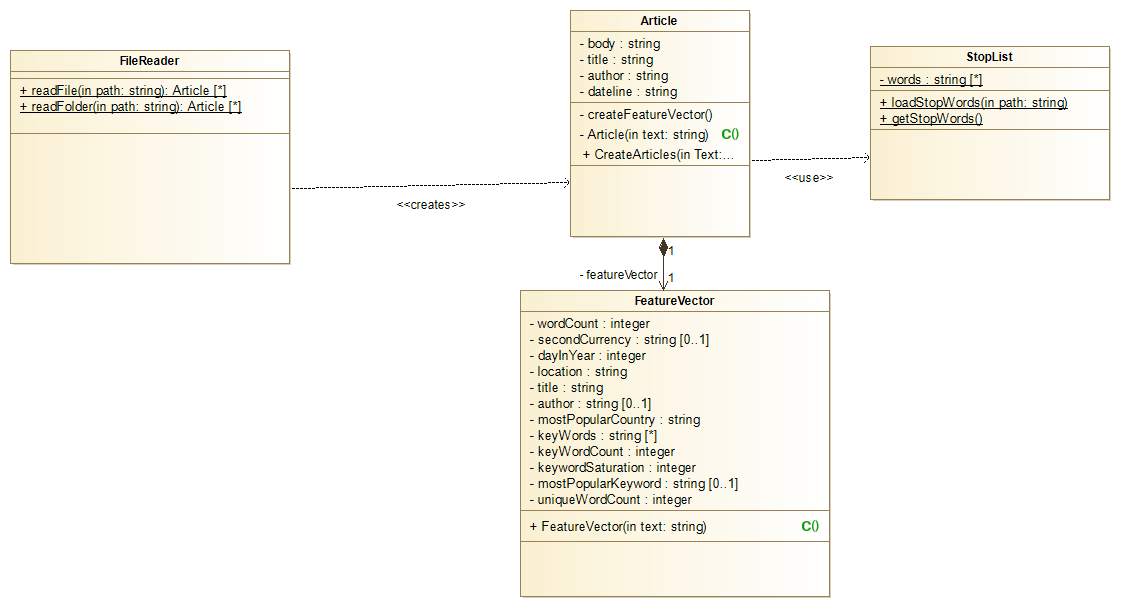
\includegraphics[width=14cm]{Ekstrakcja.png}
 \vspace{-0.3cm}
 \caption{Diagram klas modułu ekstrakcji cech. }
 \label{rysunek do eksperymentu 1 wariantu 1}
\end{figure}
\newpage

Moduł klasyfikacji oblicza odległości pomiędzy artykułem zadanym a każdym z artykułów ze zbioru trenującego za pomocą jednej z zadanych metryk \cite{dane} : metryki EuklidesowejUlicznej, , metryki metryki Czebyszewa. Dla cech zapisanych w postaci tekstowej ich odległość jest obliczana za pomocą podobieńśtwa kosinusowego. W ten sposób tworzone są pary zawierające artykuł i odleglość od zadanego artykułu. Następnie znajdowanych jest k najbliższych sąsiadów dla zadanego artykułu, gdzie poprzez słowo sąsiad rozumiemy artykuł ze zbioru trenującego. Ostatecznie artykuł jest klasyfikowany do klasy, której obiekty najczęściej wystąpiły wśród k najbliższych sąsiadów. 

\begin{figure}[h!]
 \centering
 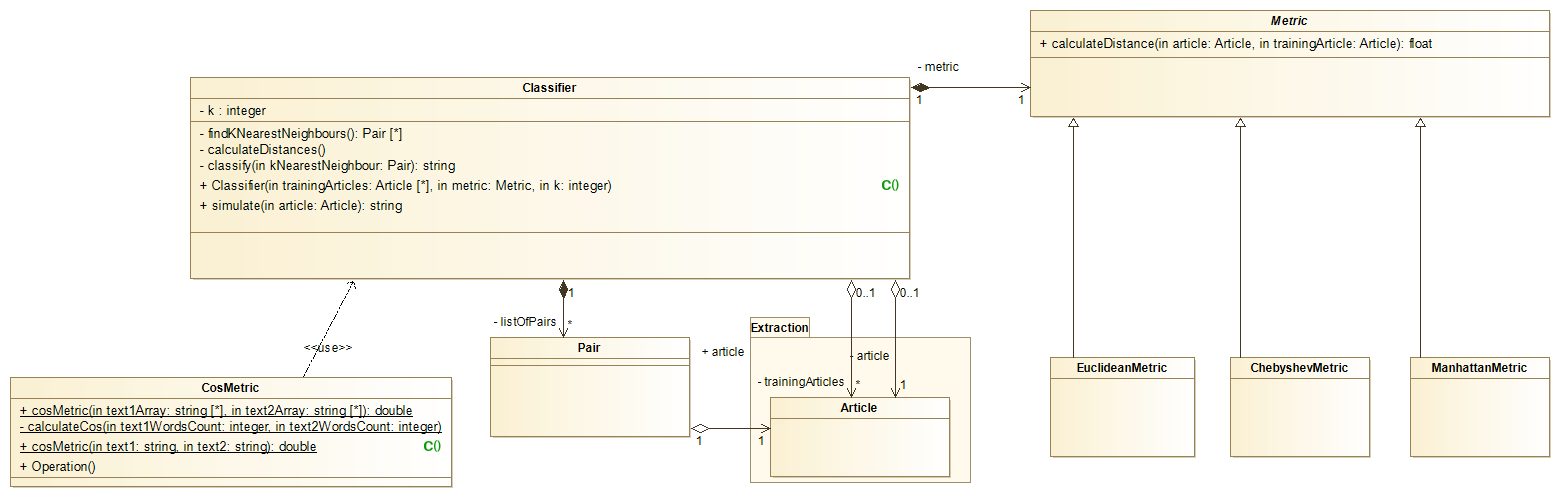
\includegraphics[width=14cm]{Klasyfikator.png}
 \vspace{-0.3cm}
 \caption{Diagram klas modułu klasyfikacji. }
 \label{rysunek do eksperymentu 1 wariantu 1}
\end{figure}

\newpage

\subsection{Prezentacja wyników, interfejs użytkownika} 
Po uruchomieniu programu użytkownik proszony jest o podanie poprzez konsolę kolejnych parametrów klasyfikacji. Na początku użytkownik podaje wartość parametru k, następnie wybiera jedną z trzech metryk, kolejno podawany jest procent zbioru treningowego w stosunku do zbioru wszystkich tekstów oraz użytkownik może podac cechy tesktów do klasyfikacji.Wybór parametrów w konsoli prezentuje się:

\begin{figure}[h!]
 \centering
 \includegraphics[width=14cm]{Wybor.png}
 \vspace{-0.3cm}
 \caption{Wybór parametrów klasyfikacji przez użytkownika. }
 \label{Wybór parametrów klasyfikacji przez użytkownika. }
\end{figure}

Po wprowadzeniu przez użytkownika wszystkich parametrów klasyfikacji, rozpoczynane jest wczytywanie danych oraz wykonanie klasyfikacji. 
\begin{figure}[h!]
 \centering
 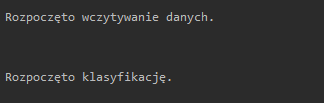
\includegraphics[width=14cm]{srodek.png}
 \vspace{-0.3cm}
 \caption{Wczytywanie danych i klasyfikacja.}
 \label{Wczytywanie danych i klasyfikacja.}
\end{figure}

Po wykonanej klasyfikacji na konsoli wyświetlany jest wynik jakości klasyfikacji oraz liczba artykułów testowych, a także liczba dobrze zklasyfikowanych artykułów. 
\begin{figure}[h!]
 \centering
 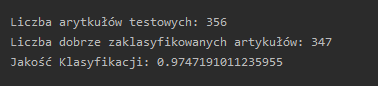
\includegraphics[width=14cm]{wynik.png}
 \vspace{-0.3cm}
 \caption{Wynik klasyfikacji.}
 \label{Wynik klasyfikacji.}
\end{figure}

Do uruchomienia programu wymagana jest wersja Javy: 11. 

\section{Wyniki klasyfikacji dla różnych parametrów wejściowych}
Wyniki kolejnych eksperymentów wg punktów 2.-8. opisu projektu 1.  Wykresy i tabele
obowiązkowe, dokładnie opisane w ,,captions'' (tytułach), konieczny opis osi i
jednostek wykresów oraz kolumn i wierszy tabel.\\ 

{**Ewentualne wyniki realizacji punktu 9. opisu Projektu 1., czyli,,na ocenę 5.0'' i ich porównanie do wyników z
części obowiązkowej**.}\\

\noindent {\bf Sekcja uzupełniona jako efekt zadania Tydzień 05 wg Harmonogramu Zajęć
na WIKAMP KSR.}


\section{Dyskusja, wnioski}
Dokładne interpretacje uzyskanych wyników w zależności od parametrów klasyfikacji
opisanych w punktach 3.-8 opisu Projektu 1. 
Szczególnie istotne są wnioski o charakterze uniwersalnym, istotne dla podobnych zadań. 
Omówić i wyjaśnić napotkane problemy (jeśli były). Każdy wniosek/problem powinien mieć poparcie
w przeprowadzonych eksperymentach (odwołania do konkretnych wyników: wykresów,
tabel). \\
\underline{Dla końcowej oceny jest to najważniejsza sekcja} sprawozdania, gdyż prezentuje poziom
zrozumienia rozwiązywanego problemu.\\

** Możliwości kontynuacji prac w obszarze systemów rozpoznawania, zwłaszcza w kontekście pracy inżynierskiej,
magisterskiej, naukowej, itp. **\\

\noindent {\bf Sekcja uzupełniona jako efekt zadania Tydzień 06 wg Harmonogramu Zajęć
na WIKAMP KSR.}


\section{Braki w realizacji projektu 1.}
Wymienić wg opisu Projektu 1. wszystkie niezrealizowane obowiązkowe elementy projektu, ewentualnie
podać merytoryczne (ale nie czasowe) przyczyny tych braków. 


\begin{thebibliography}{0}
\bibitem{dane} R. Tadeusiewicz: Rozpoznawanie obrazów, PWN, Warszawa, 1991.  
\bibitem{niewiadomski08} A. Niewiadomski, Methods for the Linguistic Summarization of Data: Applications of Fuzzy Sets and Their Extensions, Akademicka Oficyna Wydawnicza EXIT, Warszawa, 2008.

\bibitem{wyklad} A. Niewiadomski, ksr-wyklad-2009.pdf, 2009.

\bibitem{tablica} Internet forum. Wikipedia: The Free Encyclopedia, Dostępny w: \url{https://pl.wikipedia.org/wiki/Tablica_pomy%C5%82ek?fbclid=IwAR1yFbhG8HoSicSBnyA43YhpyU0tJiaIpI6ghUdNZvzDhPtMPwAWHtrdPUQ}

\bibitem{teksty} Machine Learning Repository. UCI:, Dostępny w: \url{http://archive.ics.uci.edu/ml/datasets/Reuters-21578+Text+Categorization+Collection}

\end{thebibliography}

Literatura zawiera wyłącznie źródła recenzowane i/lub o potwierdzonej wiarygodności,
możliwe do weryfikacji i cytowane w sprawozdaniu. 
\end{document}



